% Created by tikzDevice version 0.12 on 2019-03-01 10:36:22
% !TEX encoding = UTF-8 Unicode
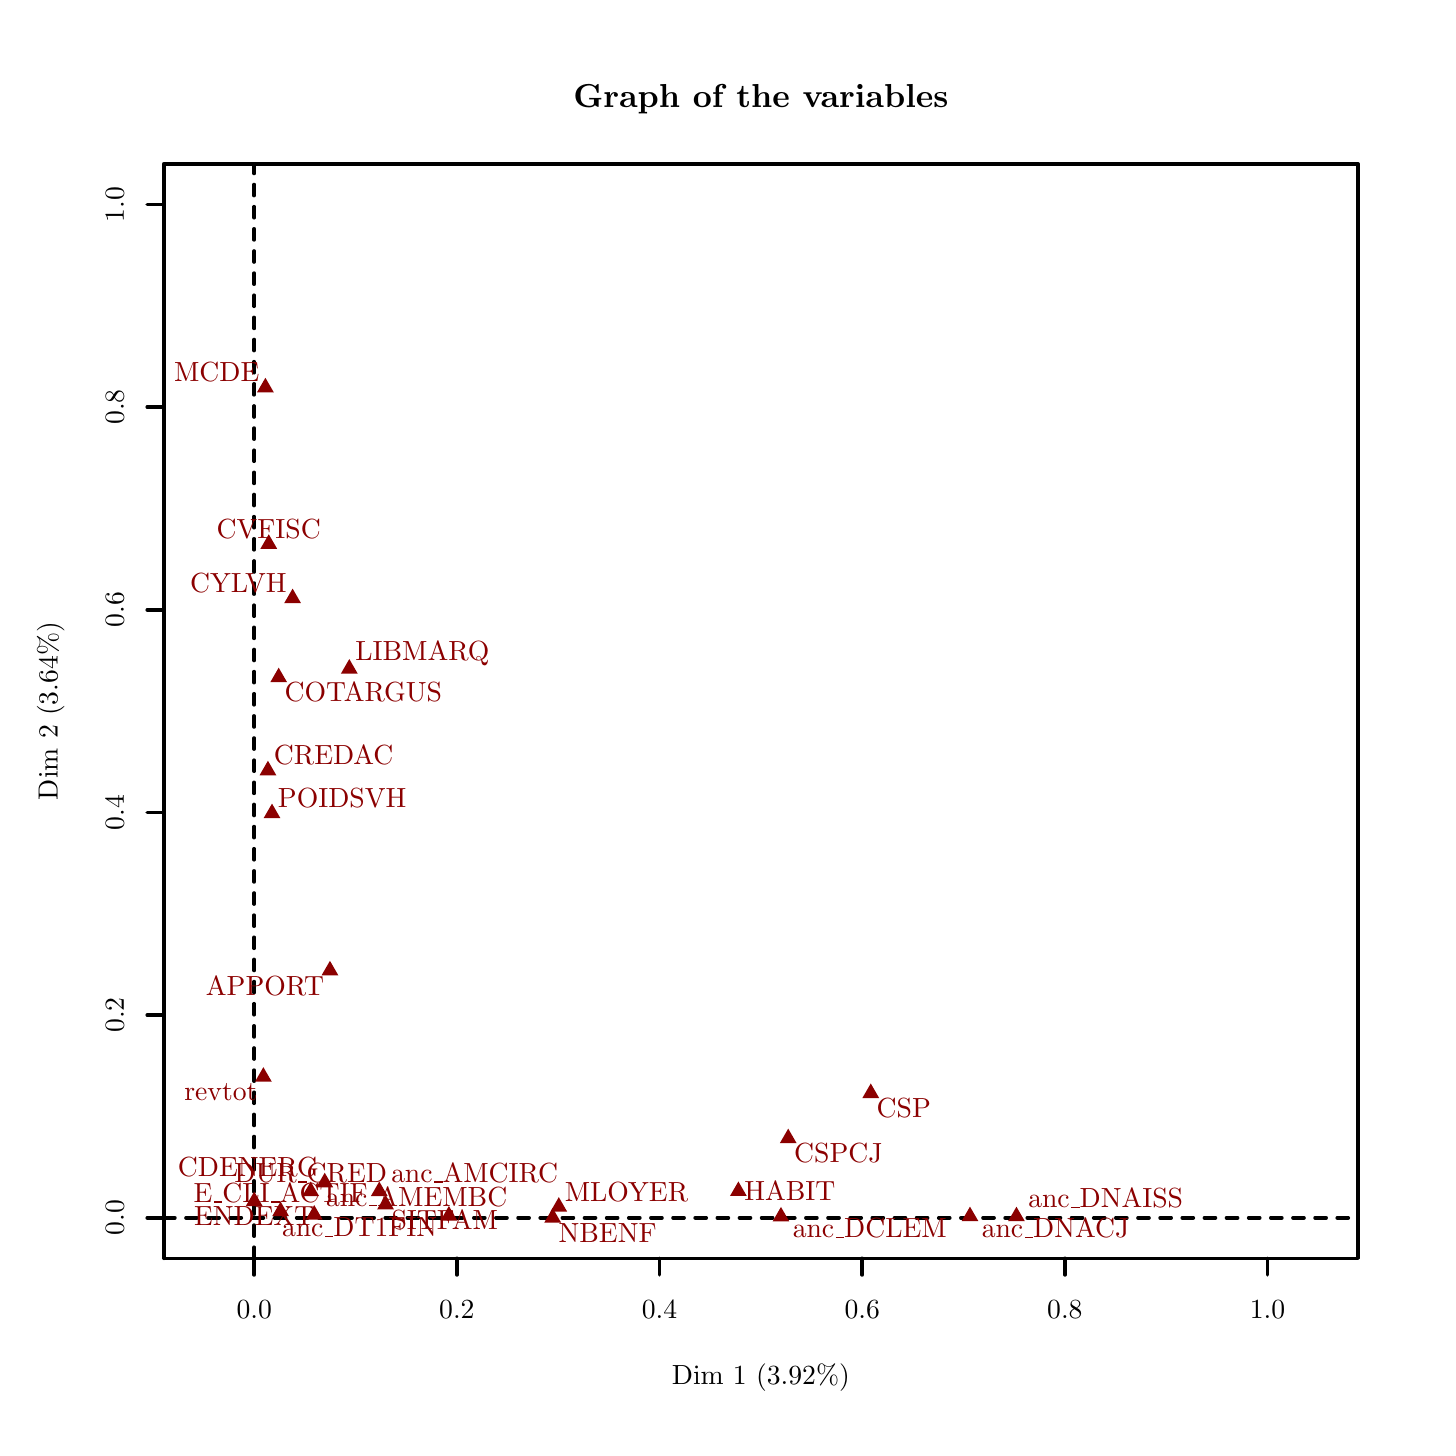
\begin{tikzpicture}[x=1pt,y=1pt]
\definecolor{fillColor}{RGB}{255,255,255}
\path[use as bounding box,fill=fillColor,fill opacity=0.00] (0,0) rectangle (505.89,505.89);
\begin{scope}
\path[clip] ( 49.20, 61.20) rectangle (480.69,456.69);
\definecolor{drawColor}{RGB}{255,255,255}

\path[draw=drawColor,line width= 1.3pt,line join=round,line cap=round] ( 81.85, 75.85) circle (  2.25);
\end{scope}
\begin{scope}
\path[clip] (  0.00,  0.00) rectangle (505.89,505.89);
\definecolor{drawColor}{RGB}{0,0,0}

\path[draw=drawColor,line width= 1.3pt,line join=round,line cap=round] ( 81.85, 61.20) -- (448.04, 61.20);

\path[draw=drawColor,line width= 1.3pt,line join=round,line cap=round] ( 81.85, 61.20) -- ( 81.85, 55.20);

\path[draw=drawColor,line width= 1.3pt,line join=round,line cap=round] (155.09, 61.20) -- (155.09, 55.20);

\path[draw=drawColor,line width= 1.3pt,line join=round,line cap=round] (228.33, 61.20) -- (228.33, 55.20);

\path[draw=drawColor,line width= 1.3pt,line join=round,line cap=round] (301.56, 61.20) -- (301.56, 55.20);

\path[draw=drawColor,line width= 1.3pt,line join=round,line cap=round] (374.80, 61.20) -- (374.80, 55.20);

\path[draw=drawColor,line width= 1.3pt,line join=round,line cap=round] (448.04, 61.20) -- (448.04, 55.20);

\node[text=drawColor,anchor=base,inner sep=0pt, outer sep=0pt, scale=  1.00] at ( 81.85, 39.60) {0.0};

\node[text=drawColor,anchor=base,inner sep=0pt, outer sep=0pt, scale=  1.00] at (155.09, 39.60) {0.2};

\node[text=drawColor,anchor=base,inner sep=0pt, outer sep=0pt, scale=  1.00] at (228.33, 39.60) {0.4};

\node[text=drawColor,anchor=base,inner sep=0pt, outer sep=0pt, scale=  1.00] at (301.56, 39.60) {0.6};

\node[text=drawColor,anchor=base,inner sep=0pt, outer sep=0pt, scale=  1.00] at (374.80, 39.60) {0.8};

\node[text=drawColor,anchor=base,inner sep=0pt, outer sep=0pt, scale=  1.00] at (448.04, 39.60) {1.0};

\path[draw=drawColor,line width= 1.3pt,line join=round,line cap=round] ( 49.20, 75.85) -- ( 49.20,442.04);

\path[draw=drawColor,line width= 1.3pt,line join=round,line cap=round] ( 49.20, 75.85) -- ( 43.20, 75.85);

\path[draw=drawColor,line width= 1.3pt,line join=round,line cap=round] ( 49.20,149.09) -- ( 43.20,149.09);

\path[draw=drawColor,line width= 1.3pt,line join=round,line cap=round] ( 49.20,222.33) -- ( 43.20,222.33);

\path[draw=drawColor,line width= 1.3pt,line join=round,line cap=round] ( 49.20,295.56) -- ( 43.20,295.56);

\path[draw=drawColor,line width= 1.3pt,line join=round,line cap=round] ( 49.20,368.80) -- ( 43.20,368.80);

\path[draw=drawColor,line width= 1.3pt,line join=round,line cap=round] ( 49.20,442.04) -- ( 43.20,442.04);

\node[text=drawColor,rotate= 90.00,anchor=base,inner sep=0pt, outer sep=0pt, scale=  1.00] at ( 34.80, 75.85) {0.0};

\node[text=drawColor,rotate= 90.00,anchor=base,inner sep=0pt, outer sep=0pt, scale=  1.00] at ( 34.80,149.09) {0.2};

\node[text=drawColor,rotate= 90.00,anchor=base,inner sep=0pt, outer sep=0pt, scale=  1.00] at ( 34.80,222.33) {0.4};

\node[text=drawColor,rotate= 90.00,anchor=base,inner sep=0pt, outer sep=0pt, scale=  1.00] at ( 34.80,295.56) {0.6};

\node[text=drawColor,rotate= 90.00,anchor=base,inner sep=0pt, outer sep=0pt, scale=  1.00] at ( 34.80,368.80) {0.8};

\node[text=drawColor,rotate= 90.00,anchor=base,inner sep=0pt, outer sep=0pt, scale=  1.00] at ( 34.80,442.04) {1.0};

\path[draw=drawColor,line width= 1.3pt,line join=round,line cap=round] ( 49.20, 61.20) --
	(480.69, 61.20) --
	(480.69,456.69) --
	( 49.20,456.69) --
	( 49.20, 61.20);
\end{scope}
\begin{scope}
\path[clip] (  0.00,  0.00) rectangle (505.89,505.89);
\definecolor{drawColor}{RGB}{0,0,0}

\node[text=drawColor,anchor=base,inner sep=0pt, outer sep=0pt, scale=  1.20] at (264.94,477.15) {\bfseries Graph of the variables};

\node[text=drawColor,anchor=base,inner sep=0pt, outer sep=0pt, scale=  1.00] at (264.94, 15.60) {Dim 1 (3.92{\%})};

\node[text=drawColor,rotate= 90.00,anchor=base,inner sep=0pt, outer sep=0pt, scale=  1.00] at ( 10.80,258.94) {Dim 2 (3.64{\%})};
\end{scope}
\begin{scope}
\path[clip] ( 49.20, 61.20) rectangle (480.69,456.69);
\definecolor{drawColor}{RGB}{0,0,0}

\path[draw=drawColor,line width= 1.3pt,dash pattern=on 4pt off 4pt ,line join=round,line cap=round] ( 81.85, 61.20) -- ( 81.85,456.69);

\path[draw=drawColor,line width= 1.3pt,dash pattern=on 4pt off 4pt ,line join=round,line cap=round] ( 49.20, 75.85) -- (480.69, 75.85);
\definecolor{drawColor}{RGB}{139,0,0}

\node[text=drawColor,anchor=base,inner sep=0pt, outer sep=0pt, scale=  1.00] at ( 85.75,156.32) {APPORT};

\node[text=drawColor,anchor=base,inner sep=0pt, outer sep=0pt, scale=  1.00] at (121.29,262.25) {COTARGUS};

\node[text=drawColor,anchor=base,inner sep=0pt, outer sep=0pt, scale=  1.00] at (110.57,239.47) {CREDAC};

\node[text=drawColor,anchor=base,inner sep=0pt, outer sep=0pt, scale=  1.00] at ( 87.12,321.31) {CVFISC};

\node[text=drawColor,anchor=base,inner sep=0pt, outer sep=0pt, scale=  1.00] at ( 76.14,301.66) {CYLVH};

\node[text=drawColor,anchor=base,inner sep=0pt, outer sep=0pt, scale=  1.00] at (102.27, 88.58) {DUR{\_{}}CRED};

\node[text=drawColor,anchor=base,inner sep=0pt, outer sep=0pt, scale=  1.00] at ( 81.86, 72.95) {ENDEXT};

\node[text=drawColor,anchor=base,inner sep=0pt, outer sep=0pt, scale=  1.00] at ( 68.33,377.86) {MCDE};

\node[text=drawColor,anchor=base,inner sep=0pt, outer sep=0pt, scale=  1.00] at (216.37, 81.78) {MLOYER};

\node[text=drawColor,anchor=base,inner sep=0pt, outer sep=0pt, scale=  1.00] at (209.57, 67.00) {NBENF};

\node[text=drawColor,anchor=base,inner sep=0pt, outer sep=0pt, scale=  1.00] at (113.63,223.98) {POIDSVH};

\node[text=drawColor,anchor=base,inner sep=0pt, outer sep=0pt, scale=  1.00] at (161.51, 88.59) {anc{\_{}}AMCIRC};

\node[text=drawColor,anchor=base,inner sep=0pt, outer sep=0pt, scale=  1.00] at (140.55, 80.09) {anc{\_{}}AMEMBC};

\node[text=drawColor,anchor=base,inner sep=0pt, outer sep=0pt, scale=  1.00] at (304.28, 68.56) {anc{\_{}}DCLEM};

\node[text=drawColor,anchor=base,inner sep=0pt, outer sep=0pt, scale=  1.00] at (389.51, 79.48) {anc{\_{}}DNAISS};

\node[text=drawColor,anchor=base,inner sep=0pt, outer sep=0pt, scale=  1.00] at (371.40, 68.68) {anc{\_{}}DNACJ};

\node[text=drawColor,anchor=base,inner sep=0pt, outer sep=0pt, scale=  1.00] at (119.92, 68.90) {anc{\_{}}DT1FIN};

\node[text=drawColor,anchor=base,inner sep=0pt, outer sep=0pt, scale=  1.00] at ( 69.81,118.27) {revtot};

\node[text=drawColor,anchor=base,inner sep=0pt, outer sep=0pt, scale=  1.00] at ( 79.73, 90.59) {CDENERG};

\node[text=drawColor,anchor=base,inner sep=0pt, outer sep=0pt, scale=  1.00] at (316.60,112.00) {CSP};

\node[text=drawColor,anchor=base,inner sep=0pt, outer sep=0pt, scale=  1.00] at (292.95, 95.68) {CSPCJ};

\node[text=drawColor,anchor=base,inner sep=0pt, outer sep=0pt, scale=  1.00] at ( 91.40, 81.33) {E{\_{}}CLI{\_{}}ACTIF};

\node[text=drawColor,anchor=base,inner sep=0pt, outer sep=0pt, scale=  1.00] at (275.42, 82.02) {HABIT};

\node[text=drawColor,anchor=base,inner sep=0pt, outer sep=0pt, scale=  1.00] at (142.61,277.19) {LIBMARQ};

\node[text=drawColor,anchor=base,inner sep=0pt, outer sep=0pt, scale=  1.00] at (150.71, 71.77) {SITFAM};
\definecolor{fillColor}{RGB}{139,0,0}

\path[fill=fillColor] (109.23,168.69) --
	(112.26,163.44) --
	(106.19,163.44) --
	cycle;

\path[fill=fillColor] ( 90.70,274.62) --
	( 93.73,269.37) --
	( 87.67,269.37) --
	cycle;

\path[fill=fillColor] ( 86.82,240.99) --
	( 89.85,235.74) --
	( 83.79,235.74) --
	cycle;

\path[fill=fillColor] ( 87.12,322.83) --
	( 90.15,317.58) --
	( 84.09,317.58) --
	cycle;

\path[fill=fillColor] ( 95.73,303.19) --
	( 98.76,297.94) --
	( 92.70,297.94) --
	cycle;

\path[fill=fillColor] (102.27, 88.94) --
	(105.30, 83.69) --
	( 99.24, 83.69) --
	cycle;

\path[fill=fillColor] ( 81.86, 85.31) --
	( 84.89, 80.07) --
	( 78.83, 80.07) --
	cycle;

\path[fill=fillColor] ( 85.90,379.38) --
	( 88.93,374.13) --
	( 82.87,374.13) --
	cycle;

\path[fill=fillColor] (191.92, 83.30) --
	(194.95, 78.05) --
	(188.89, 78.05) --
	cycle;

\path[fill=fillColor] (189.71, 79.37) --
	(192.74, 74.12) --
	(186.68, 74.12) --
	cycle;

\path[fill=fillColor] ( 88.29,225.50) --
	( 91.32,220.25) --
	( 85.26,220.25) --
	cycle;

\path[fill=fillColor] (127.06, 88.95) --
	(130.09, 83.70) --
	(124.03, 83.70) --
	cycle;

\path[fill=fillColor] (103.54, 80.45) --
	(106.57, 75.20) --
	(100.51, 75.20) --
	cycle;

\path[fill=fillColor] (272.20, 79.76) --
	(275.23, 74.51) --
	(269.17, 74.51) --
	cycle;

\path[fill=fillColor] (357.29, 79.84) --
	(360.32, 74.59) --
	(354.26, 74.59) --
	cycle;

\path[fill=fillColor] (340.50, 79.87) --
	(343.53, 74.63) --
	(337.47, 74.63) --
	cycle;

\path[fill=fillColor] (152.21, 80.10) --
	(155.24, 74.85) --
	(149.18, 74.85) --
	cycle;

\path[fill=fillColor] ( 85.17,130.27) --
	( 88.20,125.02) --
	( 82.14,125.02) --
	cycle;

\path[fill=fillColor] (107.34, 92.12) --
	(110.37, 86.87) --
	(104.31, 86.87) --
	cycle;

\path[fill=fillColor] (304.65,124.37) --
	(307.68,119.12) --
	(301.62,119.12) --
	cycle;

\path[fill=fillColor] (274.82,108.05) --
	(277.85,102.80) --
	(271.79,102.80) --
	cycle;

\path[fill=fillColor] ( 91.40, 81.69) --
	( 94.43, 76.44) --
	( 88.37, 76.44) --
	cycle;

\path[fill=fillColor] (256.81, 88.96) --
	(259.84, 83.72) --
	(253.78, 83.72) --
	cycle;

\path[fill=fillColor] (116.22,277.74) --
	(119.25,272.49) --
	(113.19,272.49) --
	cycle;

\path[fill=fillColor] (129.32, 84.14) --
	(132.35, 78.89) --
	(126.29, 78.89) --
	cycle;
\end{scope}
\end{tikzpicture}
